 \documentclass{article}
 % 3 næste linjer skal med får at vi kan skrive specialtegn såsom æ, ø og å. 
  \usepackage[T1]{fontenc}
 %% \usepackage[UTF8]{inputenc}
  \usepackage{lmodern}
  \usepackage{graphicx}

  
  \begin{document}
  
  \part*{BDSA --> OOAD \linebreak A Calendar system}
  
  \paragraph{Revision history} \mbox{}  
  
  \begin{table}[ht]
    \begin{tabular}{|p{35pt}|p{50pt}|p{150pt}|p{75pt}|}
        \hline
        Version & Date &
        Description & 
        Author         
        \\ \hline
        01.00.00 & 04-09-2012 & 
        First draft. The document fulfill the requrements for assignemt A36 - PART I &
        Nicolai Krüger 
        \\ \hline        
        01.01.00 & 18-09-2012 & 
        Added Revision history table. Started writing in english (future writing must be in english) - translation of the first version is yet to be done. & 
        Nicolai Krüger              
        \\ \hline
        01.01.01 & 04-09-2012 &
        Changed the titel of the document. \linebreak
        Removed the "use case ends" filed in the Use cases. &
        Nicolai Krüger
        \\ \hline
        01.02.00 & 23-09-2012 & 
        Translated everything to english. &
        Anders J
        \\ \hline
    \end{tabular}
\end{table}
  
  \paragraph{Vision} \mbox{} 
  
  The program has to work in a way, that it is possible to use and operate without use of a mouse. It should also be able to use without use of many shortcuts, but with a few simple and easy-to-use buttons. 
  The program also has to work on touch- and mobiledevices. 
  
   \paragraph{Use Cases}
   \begin{itemize}
   \item Create event
   	\begin{itemize}
   	\item A user starts to write a titel and/or a date of an event. 
   	\item The system then shows a live-search based on the title and/or date. Furthermore the system also shows 'a new event' formular, which the user can use if he or she wants to create a new event.   	
   	\item The user fills out as much information as he or she wants and chooses 'Create'.
   	\item The system saves the event and syncronizes with external webservers if any.
   	\item The user is shown with the created event. 
   	\item The user is shown the whole calendar (with the same viewing as before creation of the event) and the newly created event highlighted. 
   	\item Use case ends.
   	\end{itemize}
   \item Delete event
   \begin{itemize}
   	\item  A user starts to write a titel and/or a date of an event. 
   	\item The system shows a live-search for both title and date. 
   	\item The user navigates to the event that need deletion using the keyboard-arrows and clicks 'Delete'. 
   	\item The system deletes the event and syncronizes with external systems if any.
   	\item The user is shown the whole calendar, with same viewing as before the deletion.
   	\end{itemize}
   \item Edit an event
    \begin{itemize}
   	\item A user starts to write a titel and/or a date of an event.
   	\item The system shows a live-search for both title and date. 
   	\item The user navigates over to the event and clicks 'Enter'. 
   	\item The system opens the event with all fields as editable. 
   	\item The user edits the fields that he or she wants and clicks 'Save'.
   	\item The system edits the event and syncronizes with external systems if any.
   	\item The user is shown the whole calendar, with same viewing as prior to the edit. 
   	\end{itemize}
   
   \item Change viewing
   \begin{itemize}
   \item Brugeren navigere op til menuen med 4 knapper - "Dag", "Uge", "Måned" og "Indstillinger"
   \item Brugeren markere en af de 3 første knapper og trykker "enter"
   \item Systemet skifter visning af kalenderen i forhold til hvad der er trykket
   \end{itemize}
   \item Tilføje kalendere (f.eks. hotmail eller gmail)
   \begin{itemize}
   \item Brugeren navigere op til menuen med 4 knapper - "Dag", "Uge", "Måned" og "Indstillinger"
   \item Brugeren markere den sidste knap og trykker "enter"
   \item Systemet viser en liste med indstillings muligheder
   \item Brugeren vælger "Tilføj kalender"
   \item Systemet viser en formular
   \item Brugeren indtaster url til den ønskede kalenders ICS-fil, og udfylder resten af formularen og trykker "enter"
   \item Systemet forsøger at tilfå kalenderen
   \item Systemet henter data fra den nye kalender
   \item Brugeren får vist hele kalenderen (i forhold til det de fik vist før - dag, uge eller måned)
   \end{itemize}
   \item Fjern kalender
   \begin{itemize}
   \item Brugeren navigere op til menuen med 4 knapper - "Dag", "Uge", "Måned" og "Indstillinger"
   \item Brugeren markere den sidste knap og trykker "enter"
   \item Systemet viser en liste med indstillings muligheder
   \item Brugeren vælger "Slet kalender"
   \item Systemet viser en liste over kalendere som systemet henter data fra
   \item Brugeren markere den kalender som ønskes slettes og trykker "enter"
   \item Systemet beder brugeren om at bekræfte sletningen
   \item Brugeren markere "Bekræft sletning" og trykker "enter"
   \item Systemet fjerne alle relationer til kalenderen
   \item Brugeren får vist hele kalenderen (i forhold til det de fik vist før - dag, uge eller måned)
   \end{itemize}
   \item Rediger kalender
   \begin{itemize}
   \item Brugeren navigere op til menuen med 4 knapper - "Dag", "Uge", "Måned" og "Indstillinger"
   \item Brugeren markere den sidste knap og trykker "enter"
   \item Systemet viser en liste med indstillings muligheder
   \item Brugeren vælger rediger kalender
   \item Systemet viser en liste over kalendere som systemet henter data fra
   \item Brugeren markere den kalender som ønskes ændret og trykker "enter"
   \item Systemet viser en formular med udfyldte felter i forhold til den valgte kalender
   \item Brugeren ændre de felter som ønskes ændret, markere "gem" knapper og trykker "enter"
   \item Systemet opdatere med de nye informationer
   \item Brugeren får vist hele kalenderen (i forhold til det de fik vist før - dag, uge eller måned)
   \end{itemize}
   \end{itemize}
   
   \newpage 
   \paragraph{Use Case UML Diagrams} \mbox{}

   
   \begin{figure}[h]
\caption{}   
   \centering
%%   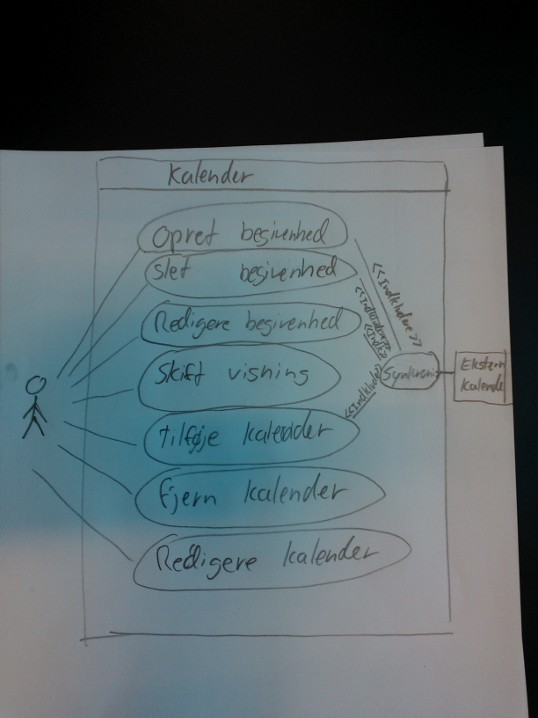
\includegraphics[scale=1.5]{WP_000143.jpg}
   \end{figure}
   
   \paragraph{Glossary} \mbox{}
\subparagraph{Begivenhed} \mbox{}

En begivenhed repræsentere en hver form for opslag i kalenderen. Aftaler, noter, arrangementer, osv. \\
Det er kort sagt den eneste ting der kan slås op, og ses i kalenderen.


   
   \paragraph{Supplementary Requirements (FURPS+)} \mbox{}
   \subparagraph{Functionality} \mbox{}
   
   \subparagraph{Error Handling} \mbox{}
   
   Alle former for fejl og exceptions, skal håndteres efter en på forhånd defineret fejlhåndterings-strategi.
   \subparagraph{Usability} \mbox{}
   
   Det skal være muligt, at anvende kalenderen uden brug af musen og kun ved hjælp af få taster.
   \subparagraph{Reliabilty} \mbox{}
   
   Kalenderen skal fungerer på en sådan måde, at den er stabil. Og hvis der skulle forekomme nedbrud, så skal kalenderen genstarte af sig selv og derved være til minimal gene for brugeren.
   \subparagraph{Performance} \mbox{}
   
   Der er ingen særlige krav til performance, udover at det skal køre flydende, som det kan forventes fra et kalendersystem i dag.
   \subparagraph{Suportability} \mbox{}
   
   
   
   
  \end{document}
